\newpage 
\section{Shifting Up (Day 3)}


\myCenteredBox[width=6in,colback=white,sharp corners,]{
    Today you will 
    \begin{itemize}[nosep,label=\checkmark]
        \item Transform yesterday's quadratic model using a vertical shift.
        \item Predict where your \mymm{}s will land when you launch from a higher place.
        \item Test your prediction.
    \end{itemize}
}

\subsection{The General Idea}

Yesterday, you found a quadratic model for your catapult:
\begin{equation*}
    y = \bm{a}(x-\bm{h})^2 + \bm{k}
\end{equation*} 

Write down the values of $\bm{a}$, $\bm{h}$, and $\bm{k}$ that you found yesterday.
\begin{tcolorbox}[colback=\myFillinColor,ams align]
    \label{a-again}
    a &= \text{\gap{???}}\\
    \label{h-again}
    h &= \text{\gap{???}}\\
    \label{k-again}
    k &= \text{\gap{???}}
\end{tcolorbox}


Today, you will use the same catapult, but you will launch 
the \mymm{}s from the a new spot located {\bfseries\itshape above} 
the floor
(one top of a desk, or a chair, or some books, or something).
This is the {\bfseries\itshape exact same catapult} 
but shifted {\bfseries\itshape vertically upward}. 

Here is a picture of the situation.
\begin{center}
    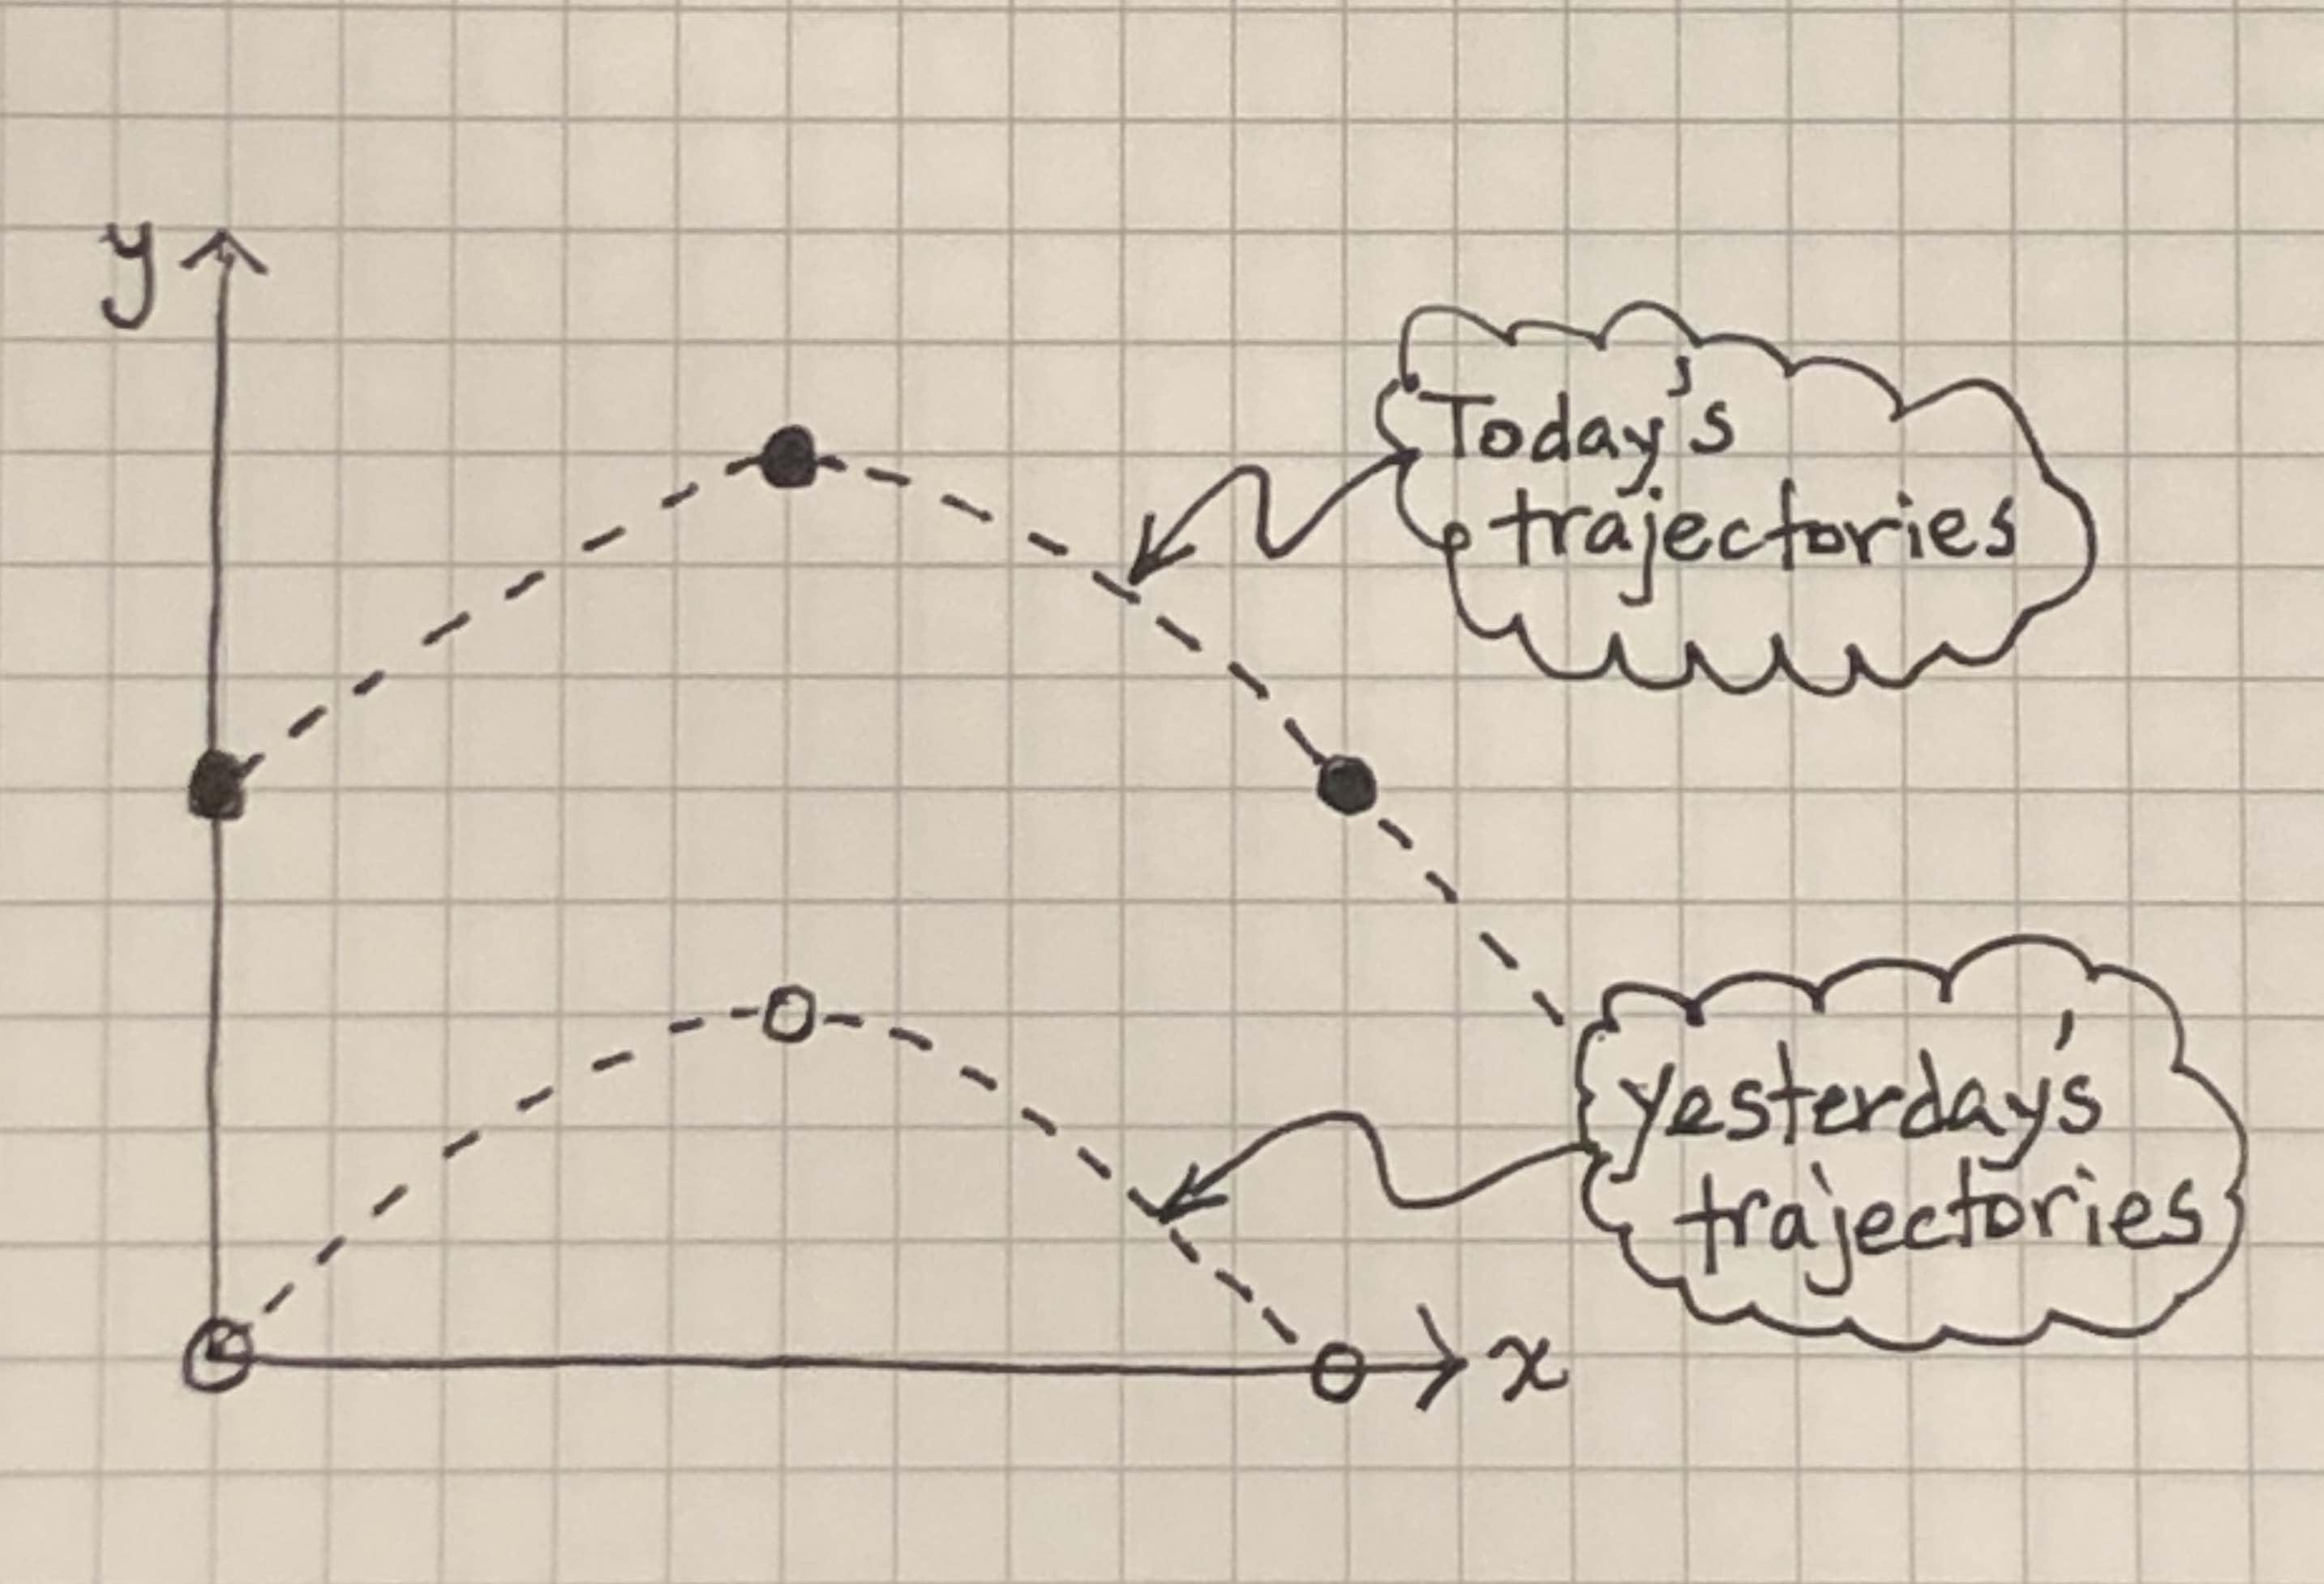
\includegraphics[width=3in]{../day1-day3-comparison.jpg}
\end{center}





\subsection{Day 3 Geometry}

As you can tell from the diagram, 
since your catapult with be higher than yesterday,
the \mymm{}s will go further.
Here is a detailed diagram of the geometry.
\begin{center}
    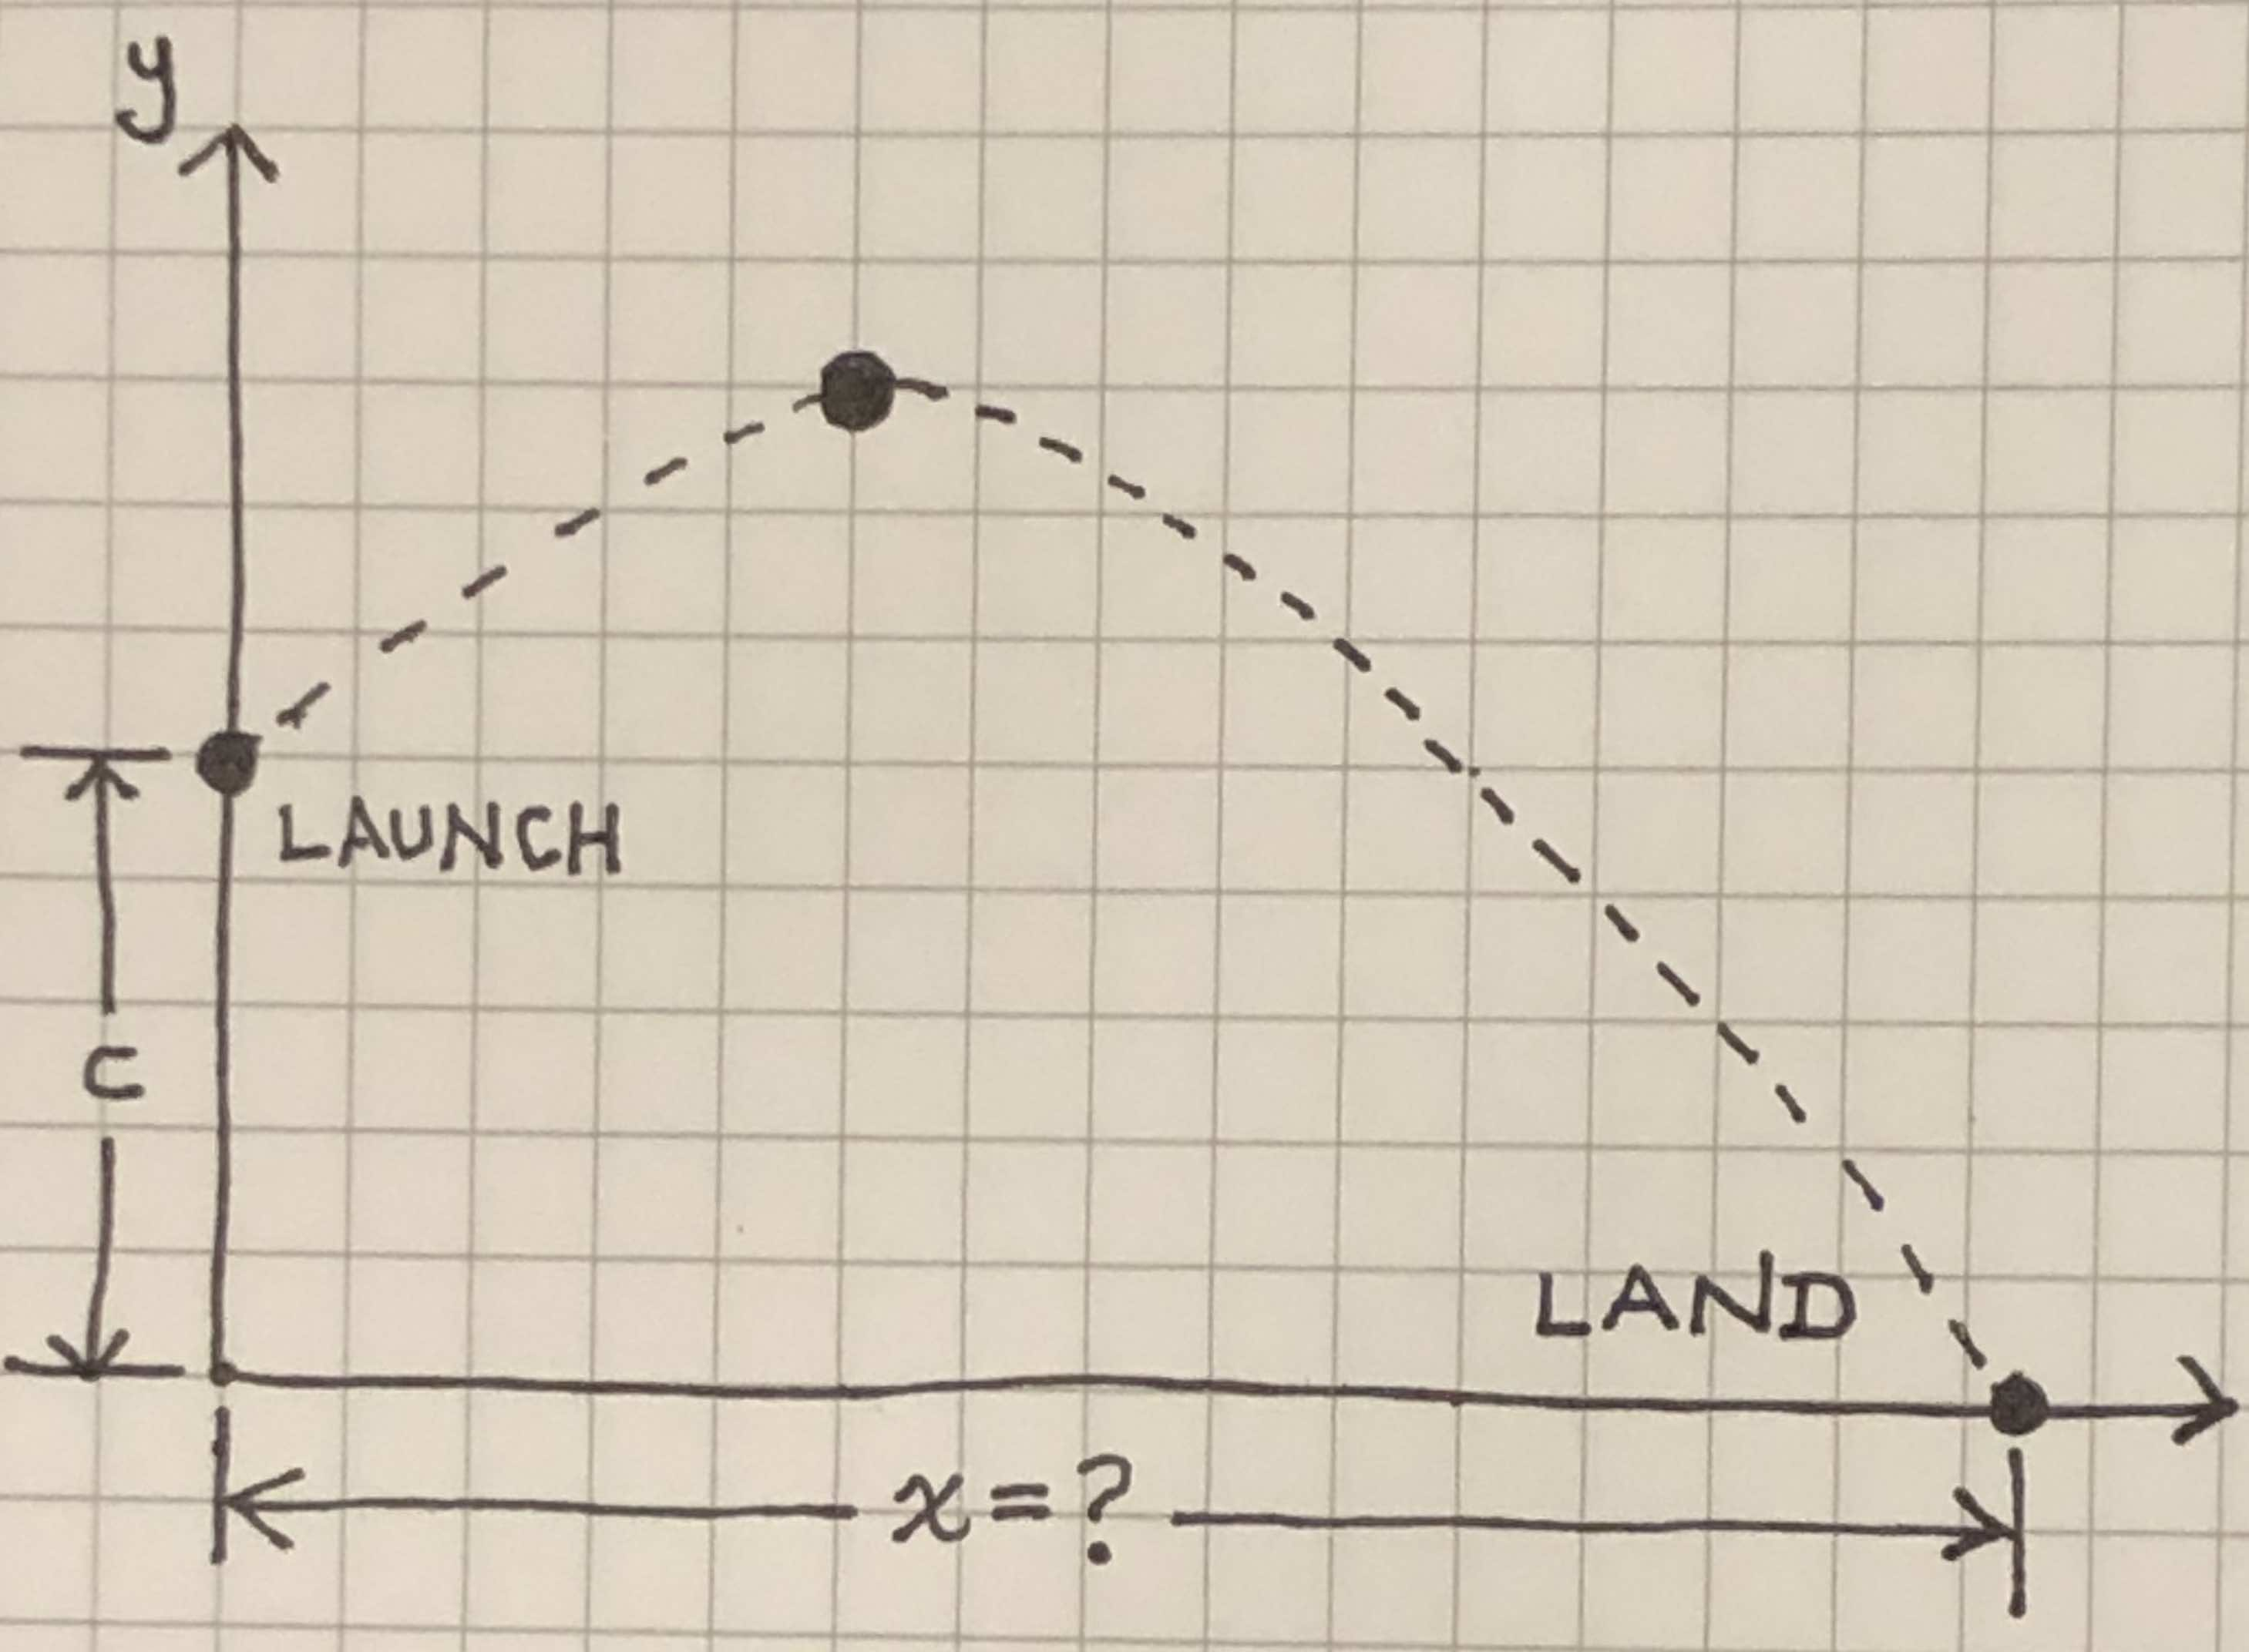
\includegraphics[width=2.5in]{../day3-geometry.jpg}
\end{center}

Your job will be to predict where your \mymm{}s will land
(to find the value of $x$).

Pick a new launch site that is above the ground.
Measure its height which is $c$.
Record that value here.
% Your group's {\bfseries\itshape measuring} person should measure how high your launch site is. 
% This is $\bm{c}$.
% The group's {\bfseries\itshape recorder} should write down your measured value.

\begin{tcolorbox}[colback=\myFillinColor,ams align]
    \label{c-value}
    c &= \text{\gap{???}}
\end{tcolorbox}





\subsection{Predicting Where The \mymm{}s Will Land}

The quadratic model for today's trajectory 
is {\itshape almost} the same as yesterday.
It's the same except for a {\bfseries\itshape vertical shift} that is added onto yesterday's equation.
$\bm{c}$ is the vertical shift.

\begin{equation}\label{shifted-model}
    y = \left[\bm{a}(x-\bm{h})^2 + \bm{k}\right] + \bm{c}
\end{equation} 

Since you know the values of $\bm{a}, \bm{h}, \bm{k}$ and $\bm{c}$,
this is an equation with two unknown variables, 
$x$ and $y$.
Evaluate this equation at the coordinates of the landing site.
Since the site is on the $x$-axis, 
it is an $x$ intercept. 
So its coordinates are 
\begin{tcolorbox}[colback=\myFillinColor,ams align]
    % (x,y)_{landing} &= (x, \text{\gap{0}}) \label{landing-site-coords} \\
    x_{landing} &= x \\
    y_{landing} &= \text{\gap{0}}
\end{tcolorbox}

Now substitute these landing site coordinates 
and the values of $\bm{a}, \bm{h}, \bm{k}$ and $\bm{c}$
into Equation~(\ref{shifted-model}).

\begin{tcolorbox}[colback=\myFillinColor,ams align]
    y_{landing} &= \left[\bm{a}(x_{landing}-\bm{h})^2 + \bm{k}\right] + \bm{c} \\
    \text{\gap{0}} &= 
        \left[
            \text{\gap{?}}
            (x-\text{\gap{?}})^2 
            + 
            \text{\gap{?}}
        \right] 
        + 
        \text{\gap{?}} 
\end{tcolorbox}

Solve this equation for $x$.
Show your work below.
(You might need to take a square root to do this. Talk to me if you need help.)
\begin{tcolorbox}[colback=\myFillinColor]
    \vspace{1.25in}
\end{tcolorbox}
\begin{tcolorbox}[colback=\myFillinColor]
    \vspace{2in}
\end{tcolorbox}

Write your value of $x$ here. 
This is your {\bfseries\itshape prediction} of where the \mymm{}s will land 
when you launch from the higher launch site.

\begin{tcolorbox}[colback=\myFillinColor,ams align]
    x &= \text{\gap{???}} \label{x-predicted}
\end{tcolorbox}





\subsection{Testing Your Prediction}

Launch \mymm{}s from you catapult three times from the higher launch site. 
Record the downrange distance for each launch.
Calculate the {\bfseries\itshape error} in your predictions 
for each launch
by subtracting your predicted value of $x$ in Equation~(\ref{x-predicted}) 
from your measured downrange distances for each launch.
\myCenteredBox[colback=\myFillinColor]{
    \centering
    \renewcommand{\arraystretch}{1.5}
    \begin{tabular}{c|p{2in}|p{2in}}
        \toprule
        {\itshape launch \#} & {\itshape downrange distance (cm)}& {\itshape error (cm)} \\
        \toprule
        1 & &\\
        \midrule
        2 & &\\
        \midrule
        3 & &\\
        \bottomrule
    \end{tabular}
}

Explain whether you think your prediction was a good one or not. 
If it was, why do you think so?
If it was not, what do you think might explain the problem?

\myCenteredBox[colback=\myFillinColor]{
    \vspace{1em}
    \underline{\hspace{\textwidth}}\\[0.5\baselineskip]
    \underline{\hspace{\textwidth}}\\[0.5\baselineskip]
    \underline{\hspace{\textwidth}}\\[0.5\baselineskip]
    \underline{\hspace{\textwidth}}\\[0.5\baselineskip]
    \underline{\hspace{\textwidth}}\\[0.5\baselineskip]
    \underline{\hspace{\textwidth}}\\[0.5\baselineskip]
    \underline{\hspace{\textwidth}}\\
}